As shown in Fig.~\ref{fig:pipeline}, our system for 3D object detection consists of three modules: frustum proposal, 3D instance segmentation, and 3D amodal bounding box estimation. We will introduce each module in the following subsections. We will focus on the pipeline and functionality of each module, and refer readers to supplementary for specific architectures of the deep networks involved.


\subsection{Frustum Proposal}
\label{sec:frustum_proposal}
%\todo{2D regions, class scores from 2D detector. lifting 2d region to point cloud in 3d frustum by backprojection of detph image patch. visualization of frustum point cloud -- foreground, background, object..}

The resolution of data produced by most 3D sensors, especially real-time depth sensors, is still lower than RGB images from commodity cameras. Therefore, we leverage mature 2D object detector to propose 2D object regions in RGB images as well as to classify objects.

With a known camera projection matrix, a 2D bounding box can be lifted to a frustum (with near and far planes specified by depth sensor range) that defines a 3D search space for the object. We then collect all points within the frustum to form a \emph{frustum point cloud}. As shown in Fig~\ref{fig:coordinate} (a), frustums may orient towards many different directions, which result in large variation in the placement of point clouds.  We therefore normalize the frustums by rotating them toward a center view such that the center axis of the frustum is orthogonal to the image plane. This normalization helps improve the rotation-invariance of the algorithm. %Note that groundtruth object orientation labels should be modified simultaneously with the frustum rotation. 
We call this entire procedure for extracting frustum point clouds from RGB-D data \emph{frustum proposal generation}.


\begin{figure}[b!]
    \centering
    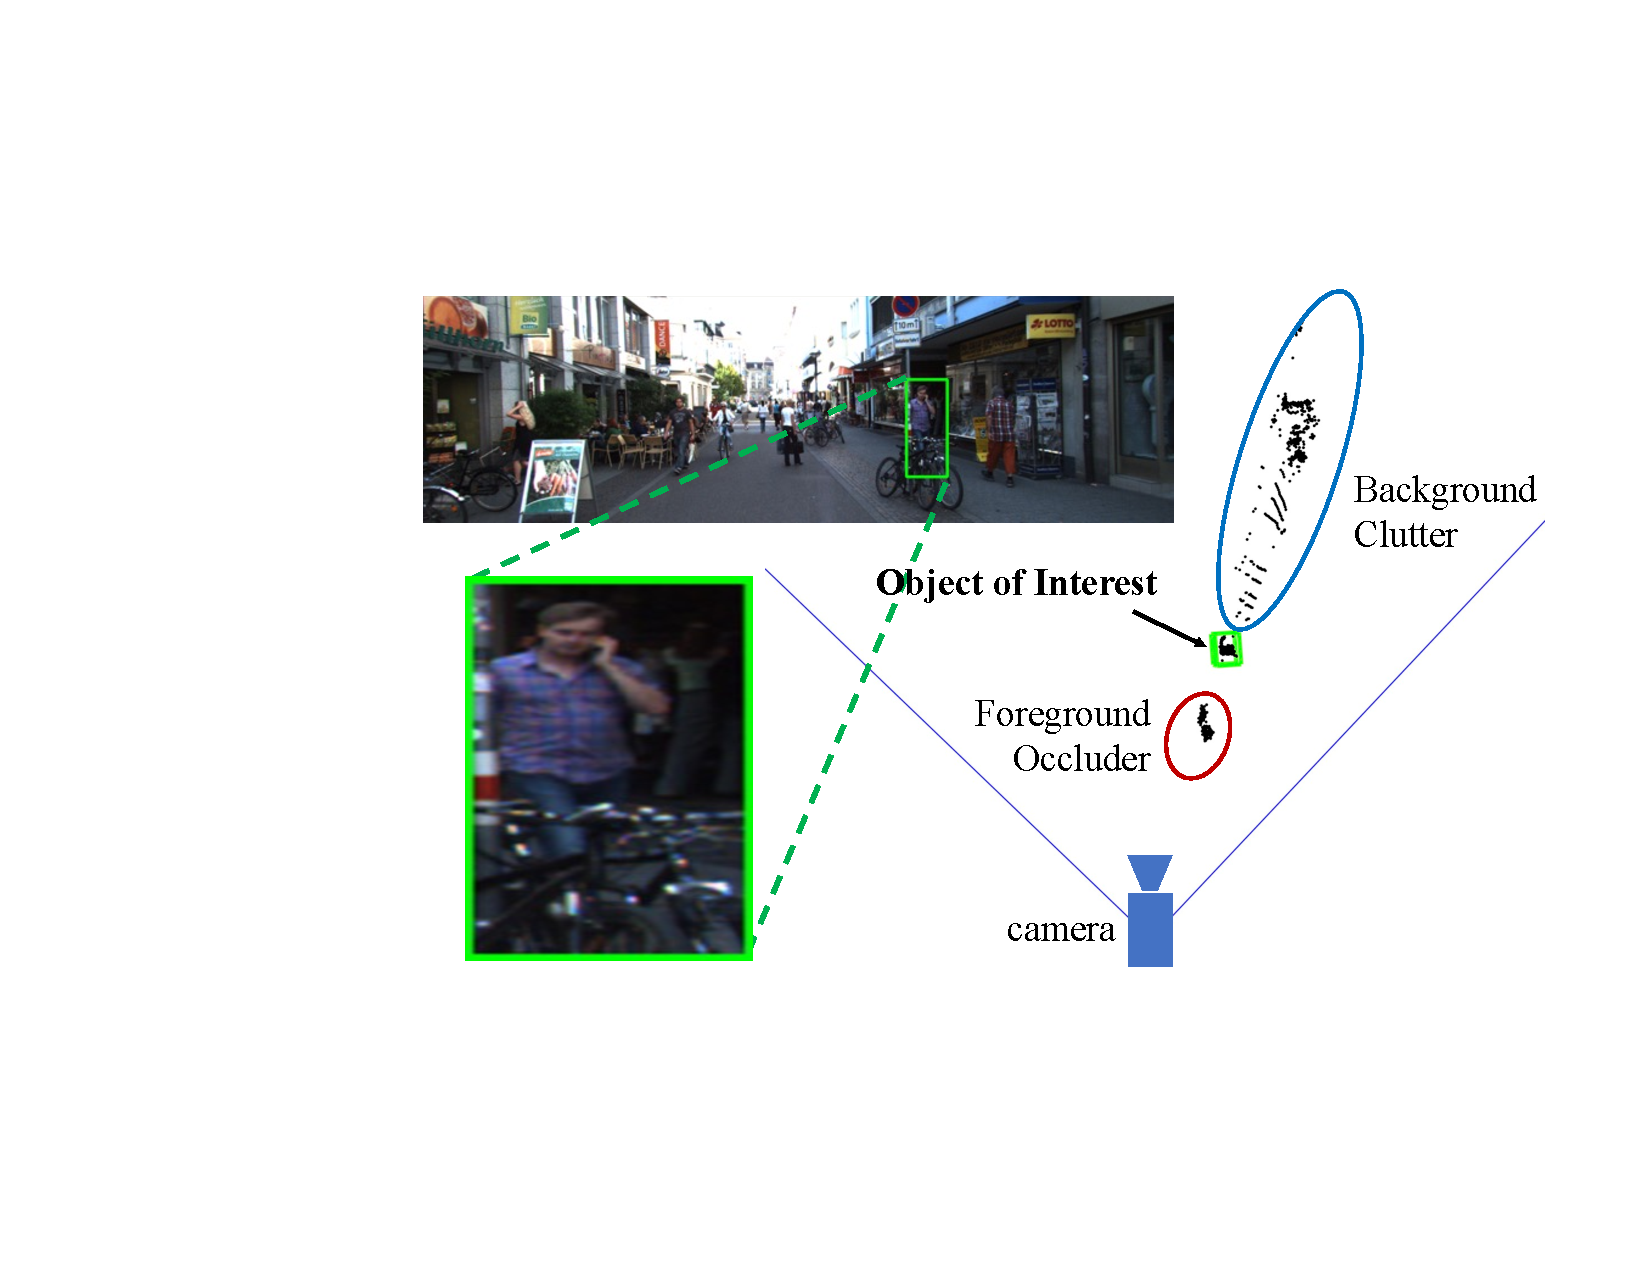
\includegraphics[width=0.8\linewidth]{fig/frustum_challenge.pdf}
    \caption{\textbf{Challenges for 3D detection in frustum point cloud.} \emph{Left:} RGB image with an image region proposal for a person. \emph{Right:} bird's eye view of the LiDAR points in the extruded frustum from 2D box, where we see a wide spread of points with both foreground occluder (bikes) and background clutter (building).}
    \label{fig:frustum}
\end{figure}


%While a 2D bounding box specifies a rough horizontal and vertical location of an object in image, the depth and 3D geometry of the object are mostly lost due to the perspective projection. In order to infer 3D location and geometry we extrude 2D boxes into 3D frustums (as illustrated in Fig.~\ref{fig:teaser}). We call this process of lifting 2D regions to 3D frustums as \emph{frustum proposal}. Then based on the point cloud living in the frustum, our next modules will localize object in 3D and estimate its bounding box.

While our 3D detection framework is agnostic to the exact method for 2D region proposal, we adopt a FPN~\cite{lin2016feature} based model. We pre-train the model weights on ImageNet classification and COCO object detection datasets and further fine-tune it on a KITTI 2D object detection dataset to classify and predict \emph{amodal} 2D boxes. More details of the 2D detector training are provided in the supplementary.


\begin{figure}[t!]
    \centering
    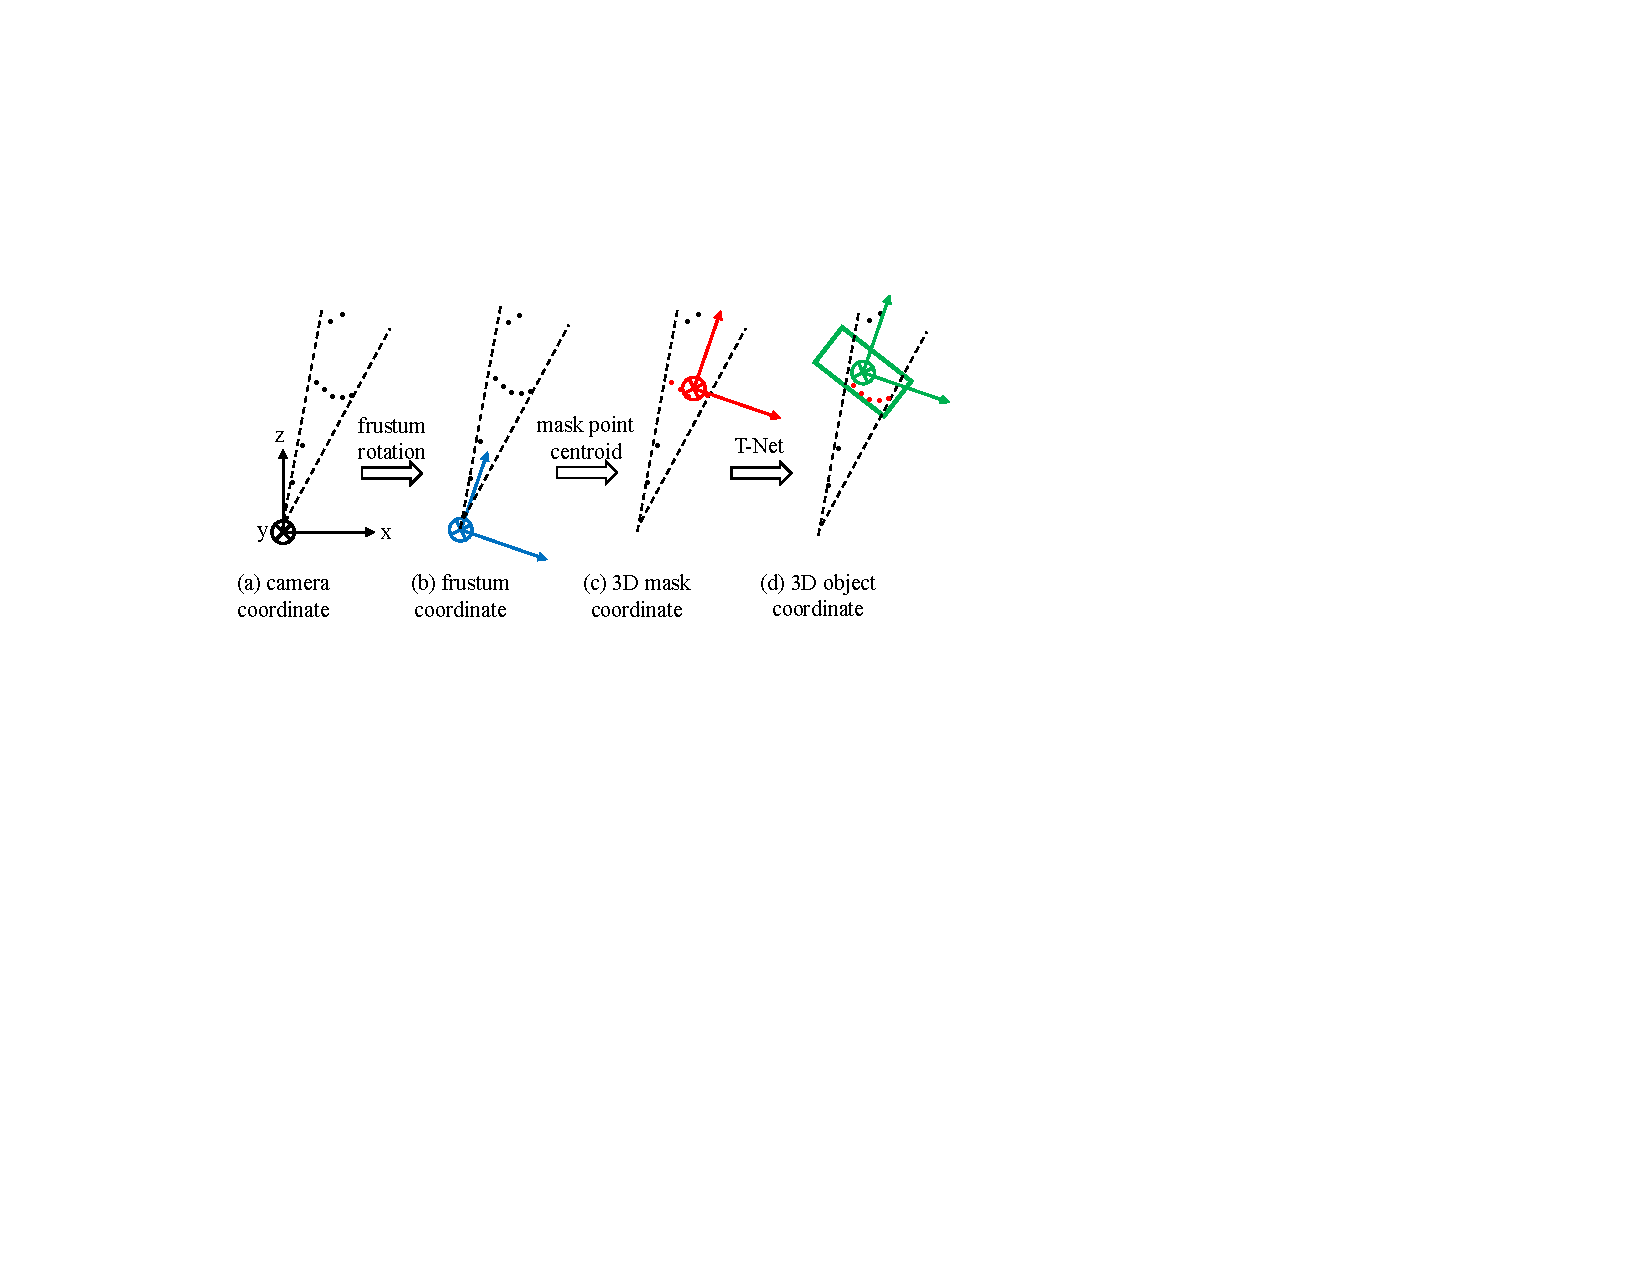
\includegraphics[width=0.95\linewidth]{fig/coordinate.pdf}
    \caption{\textbf{Coordinate systems for point cloud.} Artificial points (black dots) are shown to illustrate (a) default camera coordinate; (b) frustum coordinate after rotating frustums to center view (Sec.~\ref{sec:frustum_proposal}); (c) mask coordinate with object points' centroid at origin (Sec.~\ref{sec:instance_seg}); (d) object coordinate predicted by T-Net (Sec.~\ref{sec:box_estimation}).
    }
    \label{fig:coordinate}
\end{figure}

\subsection{3D Instance Segmentation}
\label{sec:instance_seg}
%\todo{similarity to mask r-cnn. 2d and 3d mask comparison. 3d mask segmentation as binary classification. how to support multi-class (with one-hot vector). discussion on why Fast-RCNN doesn't apply here. }

Given a 2D image region (and its corresponding 3D frustum), several methods might be used to obtain 3D location of the object:
%1) regress object depth from depth image; 2) predict 2D mask from RGB image and then regress object depth from masked depth image; 3) predict 3D mask on frustum point cloud and then regress object location in masked 3D point cloud.
One straightforward solution is to directly regress 3D object locations (e.g., by 3D bounding box) from a depth map using 2D CNNs. However, this problem is not easy as occluding objects and background clutter is common in natural scenes (as in Fig.~\ref{fig:frustum}), which may severely distract the 3D localization task. % An improved version is to apply 2D instance segmentation on RGB image (as in Mask-RCNN~\cite{he2017mask}) first and then predict depth with masked depth map.
Because objects are naturally separated in physical space, segmentation in 3D point cloud is much more natural and easier than that in images where pixels from distant objects can be near-by to each other. Having observed this fact, we propose to segment instances in 3D point cloud instead of in 2D image or depth map. Similar to Mask-RCNN~\cite{he2017mask}, which achieves instance segmentation by binary classification of pixels in image regions, we realize 3D instance segmentation using a PointNet-based network on point clouds in frustums.

Based on 3D instance segmentation, we are able to achieve \emph{residual} based 3D localization. That is, rather than regressing the absolute 3D location of the object whose offset from the sensor may vary in large ranges (e.g. from 5m to beyond 50m in KITTI data), we predict the 3D bounding box center in a local coordinate system -- 3D mask coordinates as shown in Fig.~\ref{fig:coordinate} (c).

%\paragraph{Frustum extraction and normalization} from 2D detection boxes, we firstly extract point cloud in each box-view frustum. Then an important normalization step is to align all frustums to the front with rotating them by yaw angle of the center pixel in the 2D detection box, as visualized in Fig.~\ref{fig:frustum_rotation}. The frustum alignment as a parameter-free step helps reduce distribution space of the frustum point cloud and is shown to benefit segmentation network performance.

\paragraph{3D Instance Segmentation PointNet.} The network takes a point cloud in frustum and predicts a probability score for each point that indicates how likely the point belongs to the object of interest. Note that each frustum contains exactly one object of interest. Here those ``other'' points could be points of non-relevant areas (such as ground, vegetation) or other instances that occlude or are behind the object of interest. Similar to the case in 2D instance segmentation, depending on the position of the frustum, object points in one frustum may become cluttered or occlude points in another. Therefore, our segmentation PointNet is learning the occlusion and clutter patterns as well as recognizing the geometry for the object of a certain category.

%The network is built based on the PointNet architecture -- it firstly projects each point individually into a higher embedding space by shared MLP and then gets holistic frustum feature by aggregating all point embeddings by a symmetric function (max pooling). Then single point embedding and global frustum feature are combined and fed to another MLP for final binary classification. The semantic class can be encoded as a one-hot vector and be used as additional point features along with XYZ, intensity etc. A more advanced version PointNet++ can also be used to segment the point cloud, we refer the detailed architecture to our supplementary material.

In a multi-class detection case, we also leverage the semantics from a 2D detector for better instance segmentation. For example, if we know the object of interest is a pedestrian, then the segmentation network can use this prior to find geometries that look like a person. Specifically, in our architecture we encode the semantic category as a one-hot class vector ($k$ dimensional for the pre-defined $k$ categories) and concatenate the one-hot vector to the intermediate point cloud features. More details of the specific architectures are described in the supplementary.

After 3D instance segmentation, points that are classified as the object of interest are extracted (``masking'' in Fig.~\ref{fig:pipeline}). Having obtained these segmented object points, we further normalize its coordinates to boost the translational invariance of the algorithm, following the same rationale as in the frustum proposal step.  In our implementation, we transform the point cloud into a local coordinate by subtracting XYZ values by its centroid. This is illustrated in Fig.~\ref{fig:coordinate} (c). Note that we intentionally do not scale the point cloud, because the bounding sphere size of a partial point cloud can be greatly affected by viewpoints and the real size of the point cloud helps the box size estimation.

In our experiments, we find that coordinate transformations such as the one above and the previous frustum rotation are critical for 3D detection result as shown in Tab.~\ref{tab:pc_normalization}.  %In essence, it's a process of 3D coordinate transforms such that the input data are more ``canocalized'' which greatly ease the job of the learning models on top of them. Fig.~\ref{fig:frustum_rotation} summarizes the 3D transforms we applied to the frustum point cloud. \rqi{not sure if it's the right place to introduce 3D normalization and coordinates involved in 3D detection.}


%As the frustum is constructed by 2D detection box, each frustum is expected to contain only one object of interest despite occluding objects or clutter, which supports re-formulating 3D localization from a proposal problem to a segmentation problem.


\begin{figure}[t!]
    \centering
    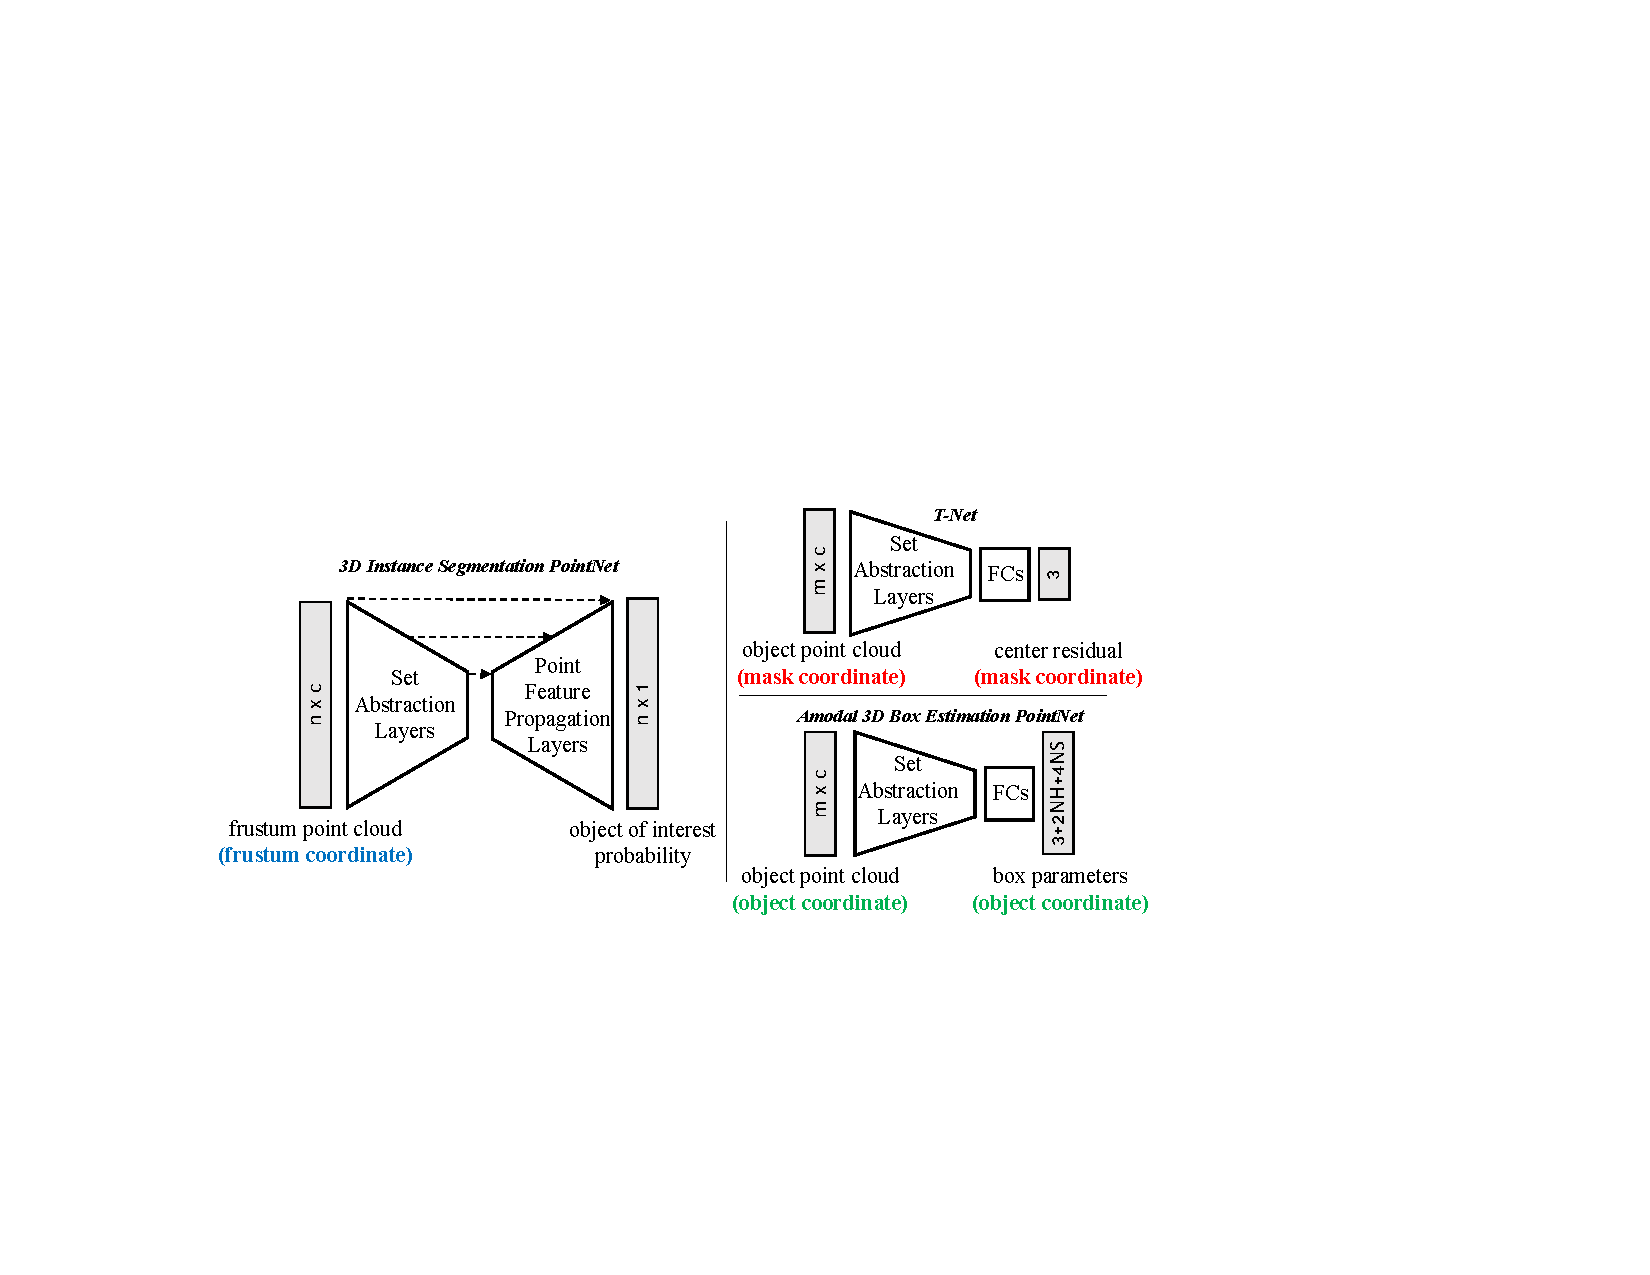
\includegraphics[width=\linewidth]{fig/network.pdf}
    \caption{\textbf{Basic architectures and IO for PointNets.} Architecture is illustrated for PointNet++~\cite{qi2017pointnetplusplus} (v2) models with set abstraction layers and feature propagation layers (for segmentation). Coordinate systems involved are visualized in Fig.~\ref{fig:coordinate}.}
    \label{fig:network}
\end{figure}

\subsection{Amodal 3D Box Estimation}
\label{sec:box_estimation}

Given the segmented object points (in 3D mask coordinate), this module estimates the object's amodal oriented 3D bounding box by using a box regression PointNet together with a preprocessing transformer network.

\paragraph{Learning-based 3D Alignment by T-Net} Even though we have aligned segmented object points according to their centroid position, we find that the origin of the mask coordinate frame (Fig.~\ref{fig:coordinate} (c)) may still be quite far from the \emph{amodal} box center. We therefore propose to use a light-weight regression PointNet (T-Net) to estimate the true center of the complete object and then transform the coordinate such that the predicted center becomes the origin (Fig.~\ref{fig:coordinate} (d)).

The architecture and training of our T-Net is similar to the T-Net in \cite{qi2017pointnet}, which can be thought of as a special type of spatial transformer network (STN)~\cite{jaderberg2015spatial}. However, different from the original STN that has no direct supervision on transformation, we explicitly supervise our translation network to predict center residuals from the mask coordinate origin to real object center. % The coordinate translation reduces the distribution space of point cloud XYZ thus allows easier optimization and enables more accurate regression to the final amodal box. Besides, note that we intentionally not to rotate the point cloud because from RGB-D data the point cloud is a partial scan -- rotated object will have different partial scan from the partial scan rotated by itself. 

\paragraph{Amodal 3D Box Estimation PointNet}
The box estimation network predicts amodal bounding boxes (for entire object even if part of it is unseen) for objects given an object point cloud in 3D object coordinate (Fig.~\ref{fig:coordinate} (d)). The network architecture is similar to that for object classification~\cite{qi2017pointnet, qi2017pointnetplusplus}, however the output is no longer object class scores but parameters for a 3D bounding box.

As stated in Sec.~\ref{sec:problem_definition}, we parameterize a 3D bounding box by its center ($c_x$, $c_y$, $c_z$), size ($h$, $w$, $l$) and heading angle $\theta$ (along up-axis). We take a ``residual'' approach for box center estimation. The center residual predicted by the box estimation network is combined with the previous center residual from the T-Net and the masked points' centroid to recover an absolute center (Eq.~\ref{eq:center}). For box size and heading angle, we follow previous works~\cite{ren2015faster, mousavian20163d} and use a hybrid of classification and regression formulations. Specifically we pre-define $NS$ size templates and $NH$ equally split angle bins. Our model will both classify size/heading ($NS$ scores for size, $NH$ scores for heading) to those pre-defined categories as well as predict residual numbers for each category ($3\times NS$ residual dimensions for height, width, length, $NH$ residual angles for heading). In the end the net outputs $3+4\times NS+2\times NH$ numbers in total.

\begin{equation}
    \label{eq:center}
    C_{pred} = C_{mask} + \Delta C_{t-net} + \Delta C_{box-net}
\end{equation}

% \begin{equation}
%     S_{pred} = T_{argmax{ss_i}} (1 + \Delta s)
% \end{equation}

% \begin{equation}
%     \theta_{pred} = \gamma_{argmax{hs_i}} + binsize \times \Delta \theta
% \end{equation}


\begin{table*}[t!]
\small
\centering
\begin{tabular}{l||ccc||ccc||ccc}
\hline
\multirow{2}{*}{Method} & \multicolumn{3}{c||}{Cars} & \multicolumn{3}{c||}{Pedestrians} & \multicolumn{3}{c}{Cyclists} \\ \cline{2-10} 
                        & Easy  & Moderate  & Hard  & Easy     & Moderate    & Hard    & Easy    & Moderate   & Hard   \\ \hline
%CSoR~\cite{Plotkin2015} & 6.76 & 6.79 & 6.14 & - & - & - & - & - & - \\
DoBEM~\cite{yuvehicle} & 7.42 & 6.95 & 13.45 & - & - & - & - & - & - \\
%MV3D (LiDAR)~\cite{cvpr17chen} & 66.77 & 52.73 & 51.31 & - & - & - & - & - & - \\
MV3D~\cite{cvpr17chen} & 71.09 & 62.35 & 55.12 & - & - & - & - & - & - \\ \hline
%AVOD (anon.)~\cite{kitti-3d-detection} & 71.41 & 62.87 & 56.61 & 29.45 & 23.42 & 22.22 & 35.94 & 29.04 & 26.44 \\ \hline
%Ours (pointnet++) & 81.04 & 65.69 & 61.68 &          &             &         &         &            &        \\ 
Ours (v1) & 80.62 & 64.70 & 56.07 & 50.88 & 41.55 & 38.04 & 69.36 & 53.50 & 52.88 \\
Ours (v2) & \textbf{81.20} & \textbf{70.39} & \textbf{62.19} & \textbf{51.21} & \textbf{44.89} & \textbf{40.23} & \textbf{71.96} & \textbf{56.77} & \textbf{50.39} \\ \hline
\end{tabular}
\caption{\textbf{3D object detection} \emph{3D} AP on KITTI \emph{test} set. DoBEM~\cite{yuvehicle} and MV3D~\cite{cvpr17chen} (previous state of the art) are based on 2D CNNs with bird's eye view LiDAR image.
%AVOD is an anonymous submission using aggregated view features and was at the top place in KITTI leader board~\cite{kitti-3d-detection} before we submitted.
Our method, without sensor fusion or multi-view aggregation, outperforms those methods by large margins on all categories and data subsets. 3D bounding box IoU threshold is 70\% for cars and 50\% for pedestrians and cyclists.}
\label{tab:kitti_test_3d_detection}
\end{table*}

\begin{table*}[t!]
\small
\centering
\begin{tabular}{l||ccc||ccc||ccc}
\hline
\multirow{2}{*}{Method} & \multicolumn{3}{c||}{Cars} & \multicolumn{3}{c||}{Pedestrians} & \multicolumn{3}{c}{Cyclists} \\ \cline{2-10} 
                        & Easy  & Moderate  & Hard  & Easy     & Moderate    & Hard    & Easy    & Moderate   & Hard   \\ \hline
%CSoR~\cite{Plotkin2015} & 23.94 & 18.69 & 16.30 & - & - & - & - & - & - \\
DoBEM~\cite{yuvehicle} & 36.49 & 36.95 & 38.10 & - & - & - & - & - & - \\
3D FCN~\cite{li20163d} & 69.94 & 62.54 & 55.94 & - & - & - & - & - & - \\
%MV3D (LiDAR)~\cite{cvpr17chen} & 85.82 & 77.00 & 68.94 & - & - & - & - & - & - \\
MV3D~\cite{cvpr17chen} & 86.02 & 76.90 & 68.49 & - & - & - & - & - & - \\ \hline
%AVOD (anon.)~\cite{kitti-3d-localization} & 85.51 & 77.57 & 69.65 & 37.53 & 30.46 & 28.30 & 44.06 & 37.11 & 32.74 \\
%NVLidarNet~\cite{kitti-3d-localization} & 84.44 & 80.04 & 74.31 & 45.21 & 37.81 & 33.82 & 63.95 & 47.97 & 44.51 \\ \hline
%Ours (pointnet++) & 81.04 & 65.69 & 61.68 &          &             &         &         &            &        \\ 
Ours (v1) & 87.28 & 77.09 & 67.90 & 55.26 & 47.56 & 42.57 & 73.42 & 59.87 & 52.88 \\
Ours (v2) & \textbf{88.70} & \textbf{84.00} & \textbf{75.33} & \textbf{58.09} & \textbf{50.22} & \textbf{47.20} & \textbf{75.38} & \textbf{61.96} & \textbf{54.68} \\ \hline
\end{tabular}
\caption{\textbf{3D object localization} AP (bird's eye view) on KITTI \emph{test} set.
%DoBEM~\cite{yuvehicle} and MV3D~\cite{cvpr17chen} are based on 2D CNNs with bird's eye view LiDAR image.
3D FCN~\cite{li20163d} uses 3D CNNs on voxelized point cloud and is far from real-time. MV3D~\cite{cvpr17chen} is the previous state of the art.
%AVOD and NVLidarNet are unpublished submissions that were at top places on KITTI leader board~\cite{kitti-3d-localization} before we submitted.
Our method significantly outperforms those methods on all categories and data subsets. Bird's eye view 2D bounding box IoU threshold is 70\% for cars and 50\% for pedestrians and cyclists.}
\label{tab:kitti_test_3d_localization}

\end{table*}

\subsection{Training with Multi-task Losses}
\label{sec:losses}

We simultaneously optimize the three nets involved (3D instance segmentation PointNet, T-Net and amodal box estimation PointNet) with multi-task losses (as in Eq.~\ref{eq:losses}).
$L_{c1-reg}$ is for T-Net and $L_{c2-reg}$ is for center regression of box estimation net. $L_{h-cls}$ and $L_{h-reg}$ are losses for heading angle prediction while $L_{s-cls}$ and $L_{s-reg}$ are for box size.
Softmax is used for all classification tasks and smooth-$l_1$ (huber) loss is used for all regression cases.

%At inference time we compute prediction box by taking size and heading class with the highest scores. The predicted center is calculated from the sum of residual centers from 3DAlignNet and box estimation net and the centroid of the segmented object points.
\vspace{-1mm}
\begin{equation}
\small
\label{eq:losses}
\begin{split}
    L_{multi-task} = & L_{seg} + \lambda (L_{c1-reg} + L_{c2-reg} + L_{h-cls} + \\
    & L_{h-reg} + L_{s-cls} + L_{s-reg} + \gamma L_{corner})
\end{split}
\end{equation}

\paragraph{Corner Loss for Joint Optimization of Box Parameters}
While our 3D bounding box parameterization is compact and complete, learning is not optimized for final 3D box accuracy -- center, size and heading have \emph{separate} loss terms. Imagine cases where center and size are accurately predicted but heading angle is off -- the 3D IoU with ground truth box will then be dominated by the angle error. Ideally all three terms (center,size,heading) should be \emph{jointly} optimized for best 3D box estimation (under IoU metric).
%\rqi{is 3D IoU compute differentiable?}
To resolve this problem we propose a novel regularization loss, the \emph{corner loss}:

\vspace{-1mm}

\begin{equation} 
\small
\label{eq:corner_loss}
    L_{corner} = \sum_{i=1}^{NS} \sum_{j=1}^{NH} \delta_{ij} \text{min} \{ \sum_{k=1}^{8} \| P_{k}^{ij} - P_{k}^{*}\|, \sum_{i=1}^{8} \| P_{k}^{ij} - P_{k}^{**} \| \}
\end{equation}

In essence, the corner loss is the sum of the distances between the eight corners of a predicted box and a ground truth box. Since corner positions are jointly determined by center, size and heading, the corner loss is able to regularize the multi-task training for those parameters.
%\rqi{is IoU and corner loss strictly decreasing or increasing in monocular order to each other?}.

To compute the corner loss, we firstly construct $NS \times NH$ ``anchor'' boxes from all size templates and heading angle bins. The anchor boxes are then translated to the estimated box center. We denote the anchor box corners as $P_k^{ij}$, where $i$, $j$, $k$ are indices for the size class, heading class, and (predefined) corner order, respectively.
%Given ground truth 3D box corners $P_k^{*}$, we compute the sum of smooth-$l_1$ distances between each of the groundtruth corner and anchor box corner.
To avoid large penalty from flipped heading estimation, we further compute distances to corners ($P_k^{**})$ from the flipped ground truth box and use the minimum of the original and flipped cases. $\delta_{ij}$, which is one for the ground truth size/heading class and zero else wise, is a two-dimensional mask used to select the distance term we care about.

%Note that the corner loss is not able to supervise heading and size classification so it's a regularization loss that cannot be used solely for box estimation net training.
%corresponding corners of predicted 3D box and groundtruth 3D box based on smooth-$l_1$ distance. However, we are not directly predicting the box corners as in MV3D~\cite{cvpr17chen}), but rather deriving predicted box corners from our compact parameterizations (i.e. center, size templates, heading bins and size/heading residuals). In that way we guarantee the box to be a strict cuboid while it is not the case for MV3D. 

%One key challenge to compute effective corner loss is to find correspondences between corners from estimated and ground truth boxes. However we can avoid finding correspondences by using the idea of ``anchor'' boxes.

%The corner loss is weighted by hyperparameter $\gamma$ and added to the final loss as a regularization. 

%As shown in our experimental evaluation (Sec.~\ref{sec:exp_analysis}), adding corner loss to our multi-task loss function significantly improves accuracy in 3D bounding box estimation.

%To compute corner distance in batch mode, we will firstly get heading candidates in each bin ($K$ headings) by combining bin center heading and residual heading estimation, similarly get size candidates for each size cluster ($M$ size options) and the estimated box center. Then we generate predicted boxes' corners for all headings and all size clusters and represent them as an array of shape $K \times M \times 8 \times 3$. Then we can construct a 2D mask matrix $S$ of shape $K \times M$ where only one element $S_{i,j}$ in the matrix is one while the others are zero -- i and j correspond to the heading and size class with higest scores respectively. By batch matrix multiplication we can extract the predicted corners as $8 \times 3$ array and then compute the corner loss by comparing it with groudtruth box as $8 \times 3$ array as well. To support mini-batch training, we can simply extend all arrays with another batch dimension.

% \todo{Wei: could we show that corner loss also helps 2D detection?}

% \begin{figure}[h]
%     \centering
%     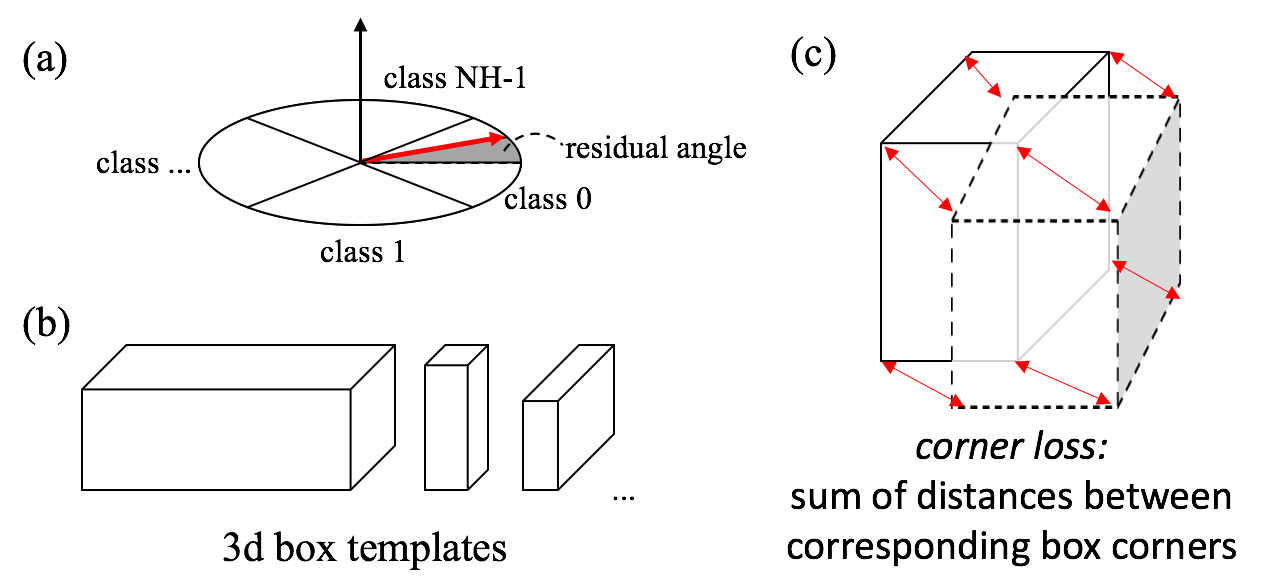
\includegraphics[width=\linewidth]{fig/box_loss}
%     \caption{3d box parameterization and loss}
% \end{figure}

%\todo{Extend the method section with some adds-on modules? such as joint bird-eye view and camera view attention. or end-to-end trainable CNN + PointNet, or 3D confidence, or 3D box proposals?}